\documentclass[a4paper]{article}
\usepackage[pdftex]{graphicx}
\usepackage[utf8]{inputenc}
\usepackage{enumerate}
\usepackage{amssymb}
\usepackage{icomma}
\usepackage{siunitx}
\sisetup{locale=DE} 
\usepackage{tikz}
\usepackage{href-ul}
\hypersetup{
	colorlinks=true,
	linkcolor=blue,
	urlcolor=blue}
\usepackage{geometry}
\geometry{a4paper, top=15mm, left=15mm, right=15mm, bottom=15mm,
	headsep=10mm, footskip=12mm}

\begin{document}
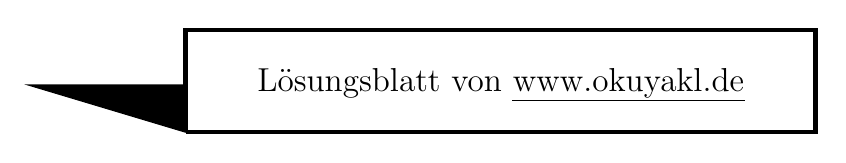
\begin{tikzpicture}(10,3)
	\draw[ultra thick](2,0) --(10,0) -- (10,1.3) --(2,1.3) -- (2,0);
	\draw[fill=black](2,0)-- (0,.6) -- (2,.6) -- (2,0);
	\node at (6,.6) {\large Lösungsblatt von \href{https://www.okuyakl.de}{www.okuyakl.de}};
\end{tikzpicture}
\vspace{0.5 cm}

\noindent{\bf Aufgabe 1. a)}\\

\begin{minipage}{0.6\textwidth}
Konstruktion der Winkelhalbierenden:
\begin{itemize}
\item  Kreis k(A;r) um A mit beliebigem Radius 
\item  Schnittpunkte von k auf den Schenkeln [AD] und [AC] markieren
\item  Kreisbögen um die Punkte miteinander schneiden
\item  Gerade durch A und den Schnittpunkt der Kreisbögen = Winkelhalbierende 
\end{itemize}

\noindent{\bf Aufgabe 1. b)}\\
Konstruktion des Rechtecks:
\begin{itemize}
\item  Strecke $\overline{DC}$ mit dem Zirkel abtragen 
\item  Kreisbogen mit diesem Radius um A 
\item  Strecke $\overline{DA}$ mit dem Zirkel abtragen 
\item  Kreisbogen mit diesem Radius um C 
\item  beide Kreisbögen schneiden = B
\item  Strecke [AB] und [CB] zeichnen.
\end{itemize}

\noindent{\bf Aufgabe 1. c)}\\
Konstruktion des Spiegelpunkts D':
\begin{itemize}
\item  Kreisbogen um D mit Achse AC zweimal schneiden
\item  Kreisbögen um die zwei Schnittpunkte
\item  Gerade durch Schnittpunkte der Kreisbögen = Lot von D auf [AC]  
\item  Länge  Punkt D -- Lotfußpunkt mit dem Zirkel abtragen
\item  Kreisbogen mit diesem Radius um L mit Geraden auf der anderen Seite schneiden = D' 
\end{itemize}
\end{minipage}
\begin{minipage}{0.4\textwidth}
\includegraphics[width= 6 cm]{dreivier249}
\includegraphics[width= 4 cm]{dreisp249}
\end{minipage}

\noindent{\bf Aufgabe 2.}\\
\begin{minipage}{0.4\textwidth}
\begin{itemize}
\item  Kreise um A und B mit beliebigem, glei\-chem Radius 
\item  Schnittpunkte der Kreise verbinden ergibt Mittelsenkrechte $m_{[AB]}$.
\item  Strecke zwischen 16 m minus 5 m = 11 m mit Zirkel abtragen. 
\item  11 m auf Mittelsenkrechte markieren ergibt Elfmeterpunkt. 
\end{itemize}
\end{minipage}
\begin{minipage}{0.6\textwidth}
\includegraphics[width=8 cm]{torelf249}\\
\end{minipage}

\noindent{\bf Aufgabe 3.}\\
Ein Dreieck ist eindeutig bestimmt durch zwei Seiten und dem Winkel, der der größeren Seite gegenüber liegt.

\noindent{\bf Aufgabe 4.}\\

\noindent
\begin{minipage}{0.7\textwidth}
	Das Dreieck $\Delta A_2 B_2 C_2 $ geht aus dem Dreieck $ \Delta A_1 B_1 C_1 $ durch Drehung im Uhrzeigersinn hervor. Folglich sind beide Dreiecke kongruent zueinander. 
\end{minipage}
\hfill
\begin{minipage}{0.3\textwidth}
	\includegraphics[width=5 cm]{pladrei053}
\end{minipage}

\noindent{\bf Aufgabe 5. a)}\\
Dieses Dreieck ist nicht konstruierbar, denn $\gamma$, der größte Winkel, liegt nicht der größten Seite gegenüber.

\noindent{\bf Aufgabe 5. b)}\\
Es ist konstruierbar, denn es gilt die Dreiecksungleichung 
$$ a+b > c; $$ 
Konstruktionsbeschreibung:
\begin{itemize}
	\item Zeichnen der Strecke [$AB$] = c 
	\item Kreis um $A$ mit Radius $\SI{6,5}{\centi\meter}$
	\item Kreis um $B$ mit Radius $\SI{3,7}{\centi\meter}$
	\item Schnittpunkt beider Kreise = $C$
	\item Zeichnen der Strecken [$AC$] und [$BC$]
\end{itemize}

\noindent{\bf Aufgabe 6.}\\
Man konstruiert zu jedem Dreieckswinkel die Winkelhalbierende. Diese schneiden sich in einem Punkt $S$. Von diesem Punkt fällt man das Lot $L$ auf eine Dreiecksseite. Wir zeichnen einen Kreis um $S$ mit dem Radius $\overline{SP}$. Dies ist der Inkreis.
\vspace{0.5 cm}


\noindent
\begin{minipage}{0.5\textwidth}
	\noindent{\bf Aufgabe 7. a)}\\
	\includegraphics[width=6 cm]{drav053}
\end{minipage}
\hfill
\begin{minipage}{0.5\textwidth}
	\noindent{\bf Aufgabe 7. b)}\\
	\includegraphics[width=6 cm]{gtra053}
\end{minipage}

\noindent{\bf Aufgabe 8.}\\

\begin{enumerate}[a)]
	\item Richtig
	\item Falsch. Gegenbeispiel: $\alpha=\beta=\gamma=80^\circ \qquad \delta=120^\circ$
	\item Falsch. Gegenbeispiel: Ein Parallelogramm ist nicht achsensymmetrisch.
	\item Falsch.  Gegenbeispiel: Ein gleichschenkliges Trapez ist nicht punktsymmetrisch.
\end{enumerate}

\newpage
\noindent{\bf Aufgabe 9.}\\

\includegraphics[width=14 cm]{neun053}

c) [$DA$] verläuft durch den zweiten und dritten Quadranten.\\

d) $d(B;g_{MC})=\SI{1,6}{\centi\meter}$\\

f) $D'(4|-1)$; liegt auf dem Kreis um M und auf der Verlängerung der Strecke [$BC$].  

\begin{center}
	\includegraphics[width=7 cm]{../../viecher/endcomic.pdf}
	
	Hier geht es zurück zum \href{https://www.okuyakl.de/math/m8dreiL053/aa053.pdf}{Aufgabenblatt}
\end{center}

\end{document}

